%--------------------------------------------------------------------------------------
% Este arquivo contém a sua introdução, objetivos e organização do trabalho
%--------------------------------------------------------------------------------------
\chapter{Introdução} \label{ch:Introdução}
    A informatização do mundo, juntamente com a evolução dos equipamentos computacionais, vem permitindo a geração e coleta de enormes volumes de dados das mais variadas fontes, podendo-se afirmar que vivemos na era dos dados \cite[p.~1]{Han:2011:DMC:1972541}.
    Grande parte dos dados criados \textit{online} está em forma de texto (escrito em linguagem natural) e um estudo feito pela Universidade da Califórnia em Berkeley em 2003 apontou, por exemplo, que somente notícias de jornais (considerando armazenamento digital do texto dos mesmos) representavam cerca de 13,5 terabytes por ano, livros cerca de 5,5 terabytes por ano, e e-mails mais de 440 exabytes por ano \cite{lyman2003much} \cite[p.~3]{Zhai2016TDMA}.
    
    A coleta e análise da sobrecarga diária de dados se apresenta como um problema que a Mineração de Texto (MT) tenta resolver no caso de dados textuais, utilizando de técnicas de mineração de dados, aprendizado de máquina, processamento de linguagem natural, Recuperação de Informação (RI) e gerenciamento do conhecimento \cite[p.~1]{Han:2011:DMC:1972541} \cite{Feldman:2006:TMH:1076381} \cite[p.~1241]{Sammut2017EMLDM}.
    Técnicas de Mineração de Texto são aplicadas na classificação e clusterização de documentos, sumarização de opiniões na internet, acesso de dados biomédicos \cite[p.~4--8]{Aggarwal_MTD_2012},
    e também em tarefas de identificação de perfis de autoria\footnotemark{} \cite[p.~906]{rangel2014overview} \cite[p.~6--7]{rangel2018overview}, auxiliando em investigações forenses linguísticas \cite{Chaski_Author_2012}. 
    
    \footnotetext{A identificação de perfis de autoria consiste na extração de características do autor com base no conteúdo e estilo do texto. Essas características podem ser gênero, faixa etária, escolaridade, entre outras \cite[p.~266]{WEREN_ARTIGO_2014}.}
    % A aplicação de técnicas de Mineração de Texto nos grandes volumes de dados
    %  e é portanto uma necessidade importante,
    
% Motivação
% Importância de MT, citar exemplos práticos (encontrar criminosos, forense ) CHECK
    % motivação informal
    % existe essa área, MT, que é útil para diversas tarefas, como por exemplo classificação de grandes volumes de texto, identificação de perfil de autor e tal.
    % ela utiliza de suporte a RI para fazer suas funções, e nas tarefas de classificação são indicados atributos do dados na representação, a engenharia de atributos permite então definir bons atributos para dados textuais
    % dentre os atributos, podem ser gerados atributos oriundos de funções de RI
    % na MT cada modelo de classificação sofre uma avaliação comparativa de desempenho, o uso de diferentes atributos impacta no desempenho do classificador
    % assim, encontrar um conjunto de atributos que melhore o desempenho de classificadores de MT é uma tarefa difícil
    % encontrar meios de melhorar o desempenho dos classificadres é um dos objetivos da MT, e utilizar novos conjuntos de atributos pode trazer avanços nesse sentido
    \begin{figure}[ht]
    \centering
    \caption{Tarefa de categorização de texto (com exemplos de treinamento disponíveis).}
    \begin{center}
        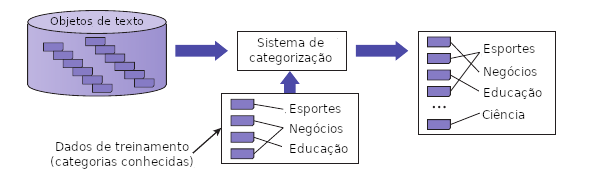
\includegraphics[width=0.75\textwidth]{img/figure15-1-zhai-traduzido.png}
    \end{center}
    \vspace{-0.5cm}
    \legend{\ABNTEXfontereduzida \textbf{Fonte:} Figura adaptada de \citeonline[p.~300]{Zhai2016TDMA}.}
    \label{fig:categorização-de-texto-zhai2016}
\end{figure}
    
    A Mineração de Texto aborda, dentre seus tipos de tarefas oriundas da mineração de dados, a tarefa de classificação nas coleções de documentos, geralmente chamada de classificação de texto ou categorização de texto \cite[p.~35]{Zhai2016TDMA}.
    Classificação é definido como o processo de designar uma ou mais categorias a cada objeto de texto, dentre categorias predefinidas, sendo que predominantemente é utilizado um conjunto de textos já classificados para treinamento \cite[p.~7]{Jo2018TMCIBDC} \cite[p.~299]{Zhai2016TDMA}.
    Este processo está exemplificado na Figura \ref{fig:categorização-de-texto-zhai2016}.
    
    No processo de classificação de texto são derivados atributos dos objetos de texto originais, um passo necessário para funcionamento do modelo de classificação proveniente da área de aprendizado de máquina \cite[p.~64]{Feldman:2006:TMH:1076381}.
    Diferentes conjuntos de atributos podem impactar diretamente no desempenho de um classificador \cite[p.~304--306]{Zhai2016TDMA}, o qual é tipicamente mensurado pela acurácia\footnotemark{} \cite[p.~313--314]{Zhai2016TDMA} \cite[p.~9]{Jo2018TMCIBDC}.
    
    \footnotetext{Número de previsões corretas dividido pelo número total de previsões feitas \cite[p.~313]{Zhai2016TDMA}.}
    
    A criação de atributos\footnotemark{} é algo que pode melhorar o acurácia dos classificadores utilizados em tarefas de mineração de dados \cite[p.~118]{MaFEDS2018}, os mesmos classificadores também são utilizados em tarefas de Mineração de Texto \cite[p.~1241]{Sammut2017EMLDM}. 
    Portanto, sugerir a criação de novos atributos, e avaliar o impacto destes atributos no desempenho de classificadores, contribui para o refinamento das técnicas de Mineração de Texto.
    Apesar de técnicas de Recuperação de Informação fundamentarem e servirem de base, principalmente, para o pré-processamento dos textos na MT, a utilização de funções de ranqueamento de RI na criação de atributos para MT é recente, sendo encontradas na literatura somente as pesquisas de \citeonline{WEREN_MESTRADO_2014}.
    
    \footnotetext{Processo da área de engenharia de atributos (\textit{feature engineering}), também chamado de extração, ou construção, de atributos \cite[p.~498--503]{Sammut2017EMLDM}.}
    
    A área de Recuperação de Informação abarca os processos de armazenamento, indexação, recuperação e ranqueamento de consultas sobre coleções de documentos \cite[p.~5--8]{Baeza-Yates2011}.
    A RI sempre busca a otimização destes processos, tanto em questão de melhoras na velocidade de resposta, como também na questão da satisfação da necessidade de informação dos usuários dos sistemas de RI \cite[p~.671--672]{Sammut2017EMLDM}, e segundo \citeonline[p.~2, tradução nossa]{KowalskiIRAA201}:
    % \begin{citacao}[english]
        % The overall goal of an Information Retrieval System is to minimize the user overhead in locating the information of value. 
        % Overhead from a user’s perspective can be defined as the time it takes to locate the needed information. 
        % The time starts when a user starts to interact with the system and ends when they have found the items of interest.
    % \end{citacao}
    
    \begin{citacao}
        O objetivo principal de um sistema de Recuperação de Informação é minimizar a sobrecarga do usuário em localizar informação de valor. 
        Na perspectiva do usuário, sobrecarga pode ser definido como o tempo que decorre para localizar a informação necessária.
        O tempo inicia quando um usuário começa a interagir com o sistema e termina quando encontra os itens de interesse.
    \end{citacao}
    Implementações de sistemas de RI que atendam os objetivos da área se tornam complexas por estes sistemas terem que lidar com a integração dos processos de forma a trazer a melhor experiência ao usuário.
    % aqui é a conclusão da parte sobre RI na introdução (após ressaltar sua complexidade):
    Portanto a utilização de ferramentas que subsidiem as tarefas de armazenamento, indexação, recuperação e ranqueamento da Recuperação de Informação, é vantajosa por assim facilitar a introdução de atributos derivados de RI nas tarefas de MT.
   
    O uso de diferentes ferramentas, para realizar a geração dos mesmos atributos derivados de RI, possibilita ainda a comparação do desempenho dessas ferramentas nas tarefas de indexação e de consulta para o ranqueamento.
    
    
    
    % A área de engenharia de atributos (tradução livre de \textit{feature engineering}) embarca a transformação, geração, extração, seleção, análise e avaliação de atributos para aprendizado de máquina
    
    % Dentre as medidas para 
    

    
    % Sistemas de RI são feitos para armazenar documentos e permitirem a sua consulta por usuários, 

% Definição do Problema
% Complexidade de RI na MT.	Dizer que RI é uma área, e vamos buscar ferramentas que subsidiam o cálculo das variáveis de RI. 

    % \section{Justificativa} \label{sec:Justificativa}
        % Existem poucos estudos na área de utilização de atributos de RI em tarefas de Mineração de Texto, também não existem (pesquisa isso) estudos do desempenho das ferramentas para subsidiar o cálculo das formulas de ranqueamento de RI. 2

    \section{Objetivo geral} \label{sec:Objetivo-geral}
        % Implementar um sistema que possibilite a utilização de atributos gerados a partir da função de ranqueamento BM25 em tarefas de Mineração de Texto.
        % Sugestão de Rosalvo
        Avaliar o desempenho de atributos oriundos de Recuperação de Informação para tarefas de Mineração de Textos.

% Avaliar o desempenho de técnicas de RI como atributos em MT
% Avaliar o desempenho de ferramentas computacionais para construção (indexação) de BDs e criação dos atributos de RI.
% Avaliar o desempenho dos classificadores de MT com e sem as var de RI.

    \section{Objetivos específicos} \label{sec:Objetivos-específicos}
        \begin{itemize}
        	\item Avaliar o ganho de desempenho de classificadores de Mineração de Texto com adição de atributos derivados da função de ranqueamento BM25 da Recuperação de Informação, em pelo menos 2 corpus de competições diferentes, utilizando medidas consolidadas na literatura;
        	
        	\item Reproduzir soluções disponíveis \textit{online} para os corpus selecionados, comprovando as medidas dos resultados das competições;
        	
            \item Elencar em qual dos corpus selecionados os atributos criados proporcionam maior ganho de desempenho de classificador;
            
            \item Comparar o desempenho computacional de ferramentas de armazenamento e indexação de textos:
            \begin{itemize}
                \item na questão de indexação;
                \item na questão de consulta utilizando as implementações do BM25 nativas das ferramentas;
            \end{itemize}
            
            \item Avaliar, empiricamente, a facilidade de instalação, utilização e integração das ferramentas de armazenamento e indexação selecionadas.
        \end{itemize}
    
    \section{Organização do trabalho} \label{sec:Organização-do-trabalho}
        Este trabalho está dividido em 3 capítulos. O primeiro capítulo é introdutório e apresenta a motivação para o desenvolvimento desta pesquisa, e qual o problema específico que o projeto aborda.
        
        No segundo capítulo é desenvolvida a fundamentação teórica dos principais campos de abordagem, sendo realizadas revisões bibliográficas das áreas de Recuperação de Informação e de Mineração de Texto.
        
        Por fim, no terceiro e último capítulo, é apresentada a metodologia para execução do projeto, ilustrada por meio de um diagrama, que é logo em seguida detalhado textualmente, e os tópicos principais são expandidos em subseções.
        No final do capítulo um cronograma de execução é apresentado, feito com base nos dias letivos do Calendário Acadêmico 2019 da UNIVASF.
% \lipsum[10-12]
